\documentclass[10pt,conference,compsocconf]{IEEEtran}

\usepackage{hyperref}
\usepackage{graphicx}	% For figure environment

% for text in math mode
\usepackage{amsmath}

% for table
\usepackage{tabu}
\usepackage{tabularx}
\usepackage{multirow}
\usepackage{subfig}

\begin{document}
\title{Sentiment Analysis of Tweets with Long Short-Term Memory Neural Networks}

\author{
  Cheng-Chun Lee, I Made Sanadhi Sutandi, Haziq Razali\\
  \textit{School of Computer and Communication Science, EPFL}
}

\maketitle

\begin{abstract}
  Deep Neural Networks have been considered as one of the most powerful machine learning methods in the last few years, forming the backbone of nearly every successful machine learning pipeline. Currently, recurrent neural networks, specifically a variant with Long Short Term Memory units (LSTM), hold state-of-the-art results in a wide range of sequence-based tasks. At a high level, they belong to the family of autoregressive models where the predicted element is conditioned on the history of inputs received thus far. In this paper, we experiment with LSTM for twitter sentiment analysis. Leveraging advances in Natural Language Processing, we show the efficacy of our algorithm with extremely competitive results.
\end{abstract}

\section{Introduction}
With the emergence of Deep Learning, Natural Language Processing (NLP) has now become a hot topic of interest and research in machine learning. The primary goal of NLP is to exploit natural language text or speech with computer application, in order to achieve something applicable for our daily lives. Combined with computational linguistic and speech technology, NLP is perpetually being used as a major component in Human Language Technologies, which aims to develop and implement appropriate tools for computer systems to understand natural languages and to execute desired tasks.

Sentiment analysis focuses on understanding how emotions, opinions, and sentiments of people are expressed in texts. Sentiment analysis is not only one part of study for Human Language Technologies, but also one of the most active research subject of NLP.  As social networks are heavily used by society, e.g. Twitter, to express opinions and emotions, the needs of leveraging advanced study of sentiment analysis starts to arise, especially for business benefits\cite{opinion_mining}.

Throughout this project, we use \textit{Long Short-Term Memory (LSTM) Neural Networks} with \textit{Global Vectors for Word Representation (GloVe)} for sentiment analysis. LSTM neural networks have been used successfully in several sequential-based tasks such as speech recognition \cite{speech_recog} and and video action recognition \cite{video_action}, and GloVe is considered better than Skip-Gram Model \cite{skip-gram}.

The rest of this report is organized as follows. In section II, we observe the tweets to reveal their properties. In section III, we list what we do in preprocessing. In section IV, we introduce GloVe embedding, which we use to map words to vectors. In section V, we describe the design of our classifier. We specify training parameters in section VI and present the results in our experiments. Lastly, we conclude and propose some possible ways to increase accuracy in section VII.

%Thus, throughout this project, we aim to develop a robust learning system capable of identifying the sentiment analysis with Twitter datasets. To achieve this, we use the Twitter large dataset of 2,500,000 tweets which consists of 1,250,000 positive and negative tweets each. Each tweet has length at most of 140 characters and usually has positive or negative smiley. Then, we test and clarify the accuracy of our model for sentiment analysis with twitter test dataset which contains 10,000 unlabeled tweets. 

\begin{figure}[t]
\begin{center}
  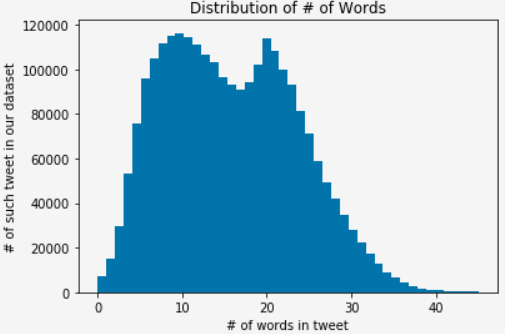
\includegraphics[width=\columnwidth]{num_words_distribution.PNG}
  \caption{Distribution of \# of words}
  \label{fig:num_words_distribution}
\end{center}
\end{figure}


\section{Observation On Dataset}
We use the Twitter large dataset of 2,500,000 tweets which consists of 1,250,000 positive and negative tweets each. Each tweet has length at most of 140 characters, and usually has positive or negative smiley. Furthermore, most of tweets consist of less than 45 words (Fig. \ref{fig:num_words_distribution}). In addition, we observe that language of tweets varies; mainly English, with some other languages like French, Malay, and so on. We clarify the accuracy of our model for sentiment analysis with twitter test dataset which contains 10,000 unlabeled tweets.

\section{Dataset Preprocessing}
Before proceeding into the training step, we perform preprocessing by removing some meaningless words and expanding or replacing words with more useful terms. The reason why we transform these words to specific words will be explained in section IV. 
\subsection{Words and Characters Removal}
Based on exploratory analysis of the training dataset, we observe some meaningless words and characteristics that give almost no information to sentiment analysis. Thus, we remove: 
\begin{itemize}
% \item \textbf{Tags} \\ There are several tags such as $<$user$>$ and $<$url$>$ in many tweets, which do not contain any meaning in the sense of sentiment.
\item \textbf{Numbers} \\
Any form of numbers as a word, such as timestamps of 23:55 and 1:20, is quite pointless for classifying the sentiments.
\item \textbf{Repeating Characters} \\
In tweets, we often see something like \textit{'exciteddddd'} or \textit{'thaaanks'}. We remove the redundant characters so that they will be considered as \textit{'excited'} and \textit{'thanks'} while doing GloVe embedding.
\end{itemize}

\subsection{Words Transformation}
In addition to removing some words and characters, we also extract some components in tweets to give more meaningful representations. Therefore, we:
\begin{itemize}
\item \textbf{Expand English Contraction} \\
In written English, contraction is frequently used, such as "I'm", "You're", "He isn't", and so on. In order to feed the words into GloVe embedding, we expand these words into "I am", "You are", "He is not", and so on.
\item \textbf{Reduce Repeated English Punctuation} \\
We reduce repeated punctuations in tweets, e.g. '!!!'.
\item \textbf{Highlight Sentiment Words} \\
Some words in English tend to have explicit emotional feelings. For instance, "\textit{convenient}" is more likely positive while "\textit{abuse}" has negative tendency. To achieve this, we utilize opinion lexicon datasets \cite{Minging}, which contain dataset of positive and negative words in English, and add "\textit{positive}" or "\textit{negative}" word before the actual word.
\item \textbf{Split Hastags({\#}) into Words} \\
Hashtag is commonly used in tweets and it is regularly used to emphasize tweets meaning. However, splitting a hashtag into undetermined number of words is a difficult task. For example, "\textit{\#meaningless}" can either be "\textit{meaningless}" or "\textit{meaning less}". To overcome this issue, we make use of word dictionary from small subset of Wikipedia and predict the words in hashtag according to frequency (pick most frequent word as possible). By dynamic programming, we split the hashtag before we map words into vectors using GloVe embedding.
\item \textbf{Transform Emojis into Special Words} \\
Based on the mouth of emoji, we can sometimes know the sentiment of this emoji. For example, ':)' usually refers to positive expression and ':(' relates to negative statement. Hence, we transform some emojis into some special words, e.g. \textit{'$<$lolface$>$'} and \textit{'$<$sadface$>$'}. However, the sentiment of emoji like ':-o' is not obvious, so we use \textit{'$<$neutralface$>$'} in this case. As we use the GloVe embedding dataset from Stanford NLP group, we need to transform some of the emojis into these special words in tweets because not all emojis are available in this dataset.
\end{itemize}

\section{GloVe Embedding}
Global Vectors for Word Representation (GloVe) \cite{GloVe} is an algorithm for mapping a word to a vector. The theory of GloVe is based on co-occurrence statistics. For instance, the co-occurrence probability of 'ice' and 'solid' is higher than that of 'ice' and 'gas'. We let machines read in several articles and measure the number of times that two words co-occur, and use subgradient descent to minimize the following function:
$$J = \sum_{i,j=1}^{V}{f(X_{ij})(w_j^T\tilde{w}_j + b_i + \tilde{b}_j - logX_{ij})^2}$$
where $f$ is the weighting function, $V$ is the size of vocabulary, $X_{ij}$ is co-occurrence probability, and $w$ and $b$ are parameters to be trained. We transform and emphasize words to sentiment words in our preprocessing so that we can more effectively use the pre-trained word vectors for tweets from Stanford NLP group \cite{GloVetweet}. This GloVe dataset includes all the transformed words, such as 'positive', $<$sadface$>$', and represents each frequent word with a 200-dimension vector. With the pre-trained word vectors, we generate a 40x200 matrix for each tweet as an input to LSTM:
$$\begin{bmatrix}
word \  vector \  of \  1st \  word \\
word \  vector \  of \  2nd \  word \\
... \\
word \  vector \  of \  39th \  word \\
word \  vector \  of \  40th \  word 
\end{bmatrix}$$

If the number of words is less than 40, then we pad 0's to the matrix. There are 2 reasons why we choose 40 as the number of rows. First is that the number of words in 99.93\% of preprocessed tweets is less than or equal to 40 (Fig. \ref{fig:num_words_distribution1}), and the second reason is that it leads to higher accuracy (Table \ref{tab:table_timesteps})

\begin{figure}[t]
\begin{center}
  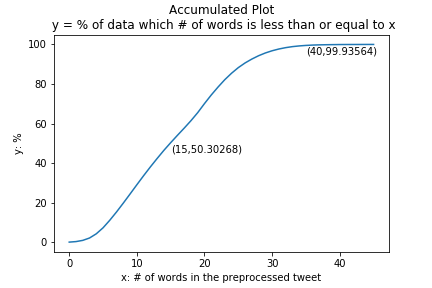
\includegraphics[width=\columnwidth]{num_words_distribution1.PNG}
  \caption{Accumulated Plot of \# of Words}
  \label{fig:num_words_distribution1}
\end{center}
\end{figure}

\section{Architecture} 

The general architecture used in this this experiment is shown in figure \ref{fig:pipeline}. At each timestep, the LSTM \cite{lstm} receives a 200-dimensional GloVe embedded word and updates its parameters via the following recurrence equation:
\begin{align*}
\textnormal{input gate} \: i_t &= sigm(W_i \cdot [x_t, h_{t-1}] + b_i) \\
\textnormal{forget gate} \: f_t &= sigm(W_f \cdot [x_t, h_{t-1}] + b_f) \\
\textnormal{output gate} \: o_t &= sigm(W_o \cdot [x_t, h_{t-1}] + b_o) \\
\textnormal{input modulation gate} \: g_t &= tanh(W_g \cdot [x_t, h_{t-1}] + b_g) \\
\textnormal{memory unit} \: c_t &= f_t \circ c_{t-1} + i_t \circ g_t \\
\textnormal{hidden unit} \: h_t &= o_t \circ tanh(c_t) \\
\end{align*}

Intuitively, the use of sigmoids at the gates allow LSTMs to control the flow of information through the unit by looking at the current input and past time-steps. We chose to use LSTMs due to its ability to learn long term dependencies, a requirement that cripples the performance of vanilla RNNs due to the problem of vanishing / exploding gradients \cite{explodingvanishinggradient1,explodingvanishinggradient2}. In our implementation, we pass a zero vector to the LSTM over the remaining timesteps for tweets that contain less than 40 words. The output at t=40 is then forwarded through 4 fully connected layers with [512,512,512,2] units before applying a sigmoid operation at the end for classification.

\begin{figure*}[t]
\begin{center}
  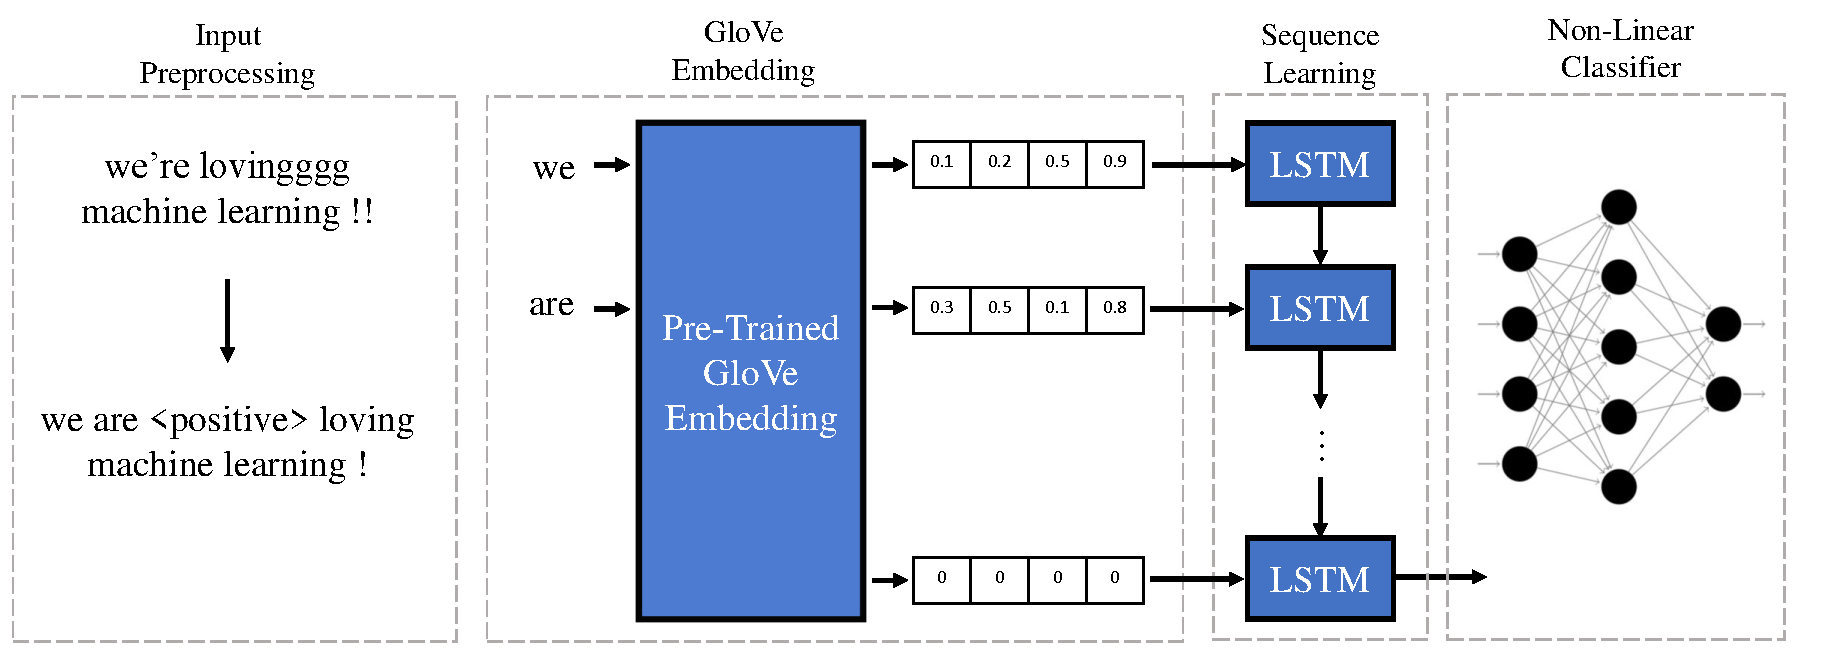
\includegraphics[width=\textwidth]{ML.pdf}
  \caption{Twitter Sentiment Analysis Pipeline}
  \label{fig:pipeline}
\end{center}
\end{figure*}

%\begin{figure*}[t]
%\begin{center}
%  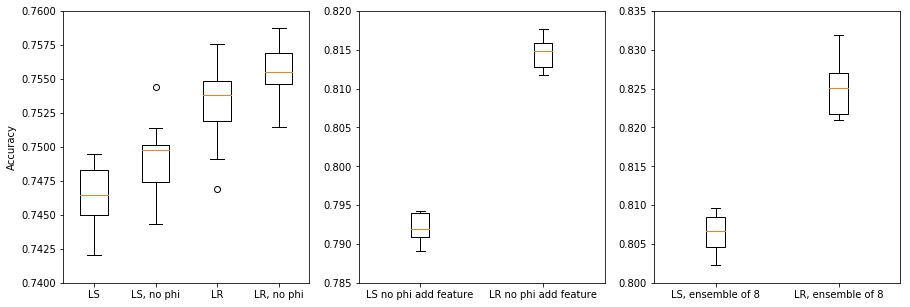
\includegraphics[width=\textwidth]{box1.jpg}
%  \caption{Box plot distributions of our models.}
%\end{center}
%   \label{fig:boxplot}
%\end{figure*}

\section{Experiments}

\subsection{Training}
We initialize all parameters using the glorot uniform initializer \cite{glorot}. Optimization is performed using stochastic gradient descent with a batch size of 1000. We use the learning scheme of RMSProp \cite{rmsprop} with a base learning rate of 5e-4, a decay of 0.9 and with no momentum. We unroll the LSTM with 1024 units for 40 time-steps and train the model for 10 epochs. The dataset is split with ratio of 90\% for training and 10\% for validation. To avoid over-fitting, we use dropout \cite{dropout} on all fully connected layers with a keep probability of 0.5. We transform the binary labels to a one-hot encoding. The experiments are run in a machine with 2 NVIDIA Titan X and takes approximately 4 hours of training time. We use the Tensorflow library \cite{tf} to develop the model. 

\subsection{Results}

In the first experiment, we evaluate the architecture described above against several baselines: Naive Bayes and a Decision Tree using the scikit library \cite{sklearn} with default parameters. Since all these algorithms require each sentence to be a feature vector, we flattened the glove embedded matrix of each word before concatenating the words to form a vector of length 8000. As expected, the performance of the LSTM surpasses all these models by a significant margin as in Table \ref{tab:baseline}. We speculate that this is due to the fact that these algorithms assume no dependence among the inputs; their output is simply a non-linear combination of all input variables. LSTMs on the other hand take advantage of the sequential structure present in language. These findings thus further corroborate the necessity of sequential processing in NLP.

% ssume the position of the words in the document doesn't matter.

In the second experiment, we study the effect of different configurations of our architecture to the accuracy. We first vary the number of fully connected layers while keeping the LSTM timesteps fixed at 40. To avoid having to experiment with an excessively large number of combinations, we simply fix each layer to have 512 units with the final classification layer at 2 units. The results have been summarized in table \ref{tab:table_fc}. It is interesting to note that largest improvement can be seen when we increase the number of layers from 3 to 4. This would make sense if we view the output of the LSTM as a feature vector representing the sentiment of the twitter post that are not linearly separable. The expressive power of the fully connected layers would thus increase with depth. Finally, we can also see that increasing the number of layers beyond 4 resulted in a degradation of accuracy. 

Next, we fix the fully connected layers at 4 layers with [512,512,512,2] units and vary the LSTM timesteps. The results have been summarized in table \ref{tab:table_timesteps}. It can be observed that reducing the number of timesteps below 40 results in a decrease in performance. This is due to the fact that the sentiment of some tweets can only be deduced towards the end of the sentence. It is also fascinating to note that increasing the number of timesteps to 45 results in a huge decrease in performance. We observe the accuracy oscillating about 65\% over the 10 epochs. It is uncertain if the number of timesteps resulted in the architecture is stuck in a local minima in early training.

%It can be observed that increasing the number of timesteps from 40 to 45 does not result in a performance gain. This can be explained with the statistics gathered in Figure 2. Since 99.93\% of the preprocessed tweets have at most 40 words, allowing the LSTM to learn for longer timesteps will not provide a noticeable gain in accuracy and can even in this case, reduce overall accuracy. Additionally, we can also see that the accuracy decreases significantly when training below 40 timesteps. This is most probably due to the fact that the sentiment of some tweets can only be deduced towards the end of the sentence.

Lastly, we display the validation accuracy plots (figure \ref{fig:accuracy}) for our second experiment and we observe that there is no clear sign of overfitting.

\begin{table}[t]
 	\small
	\begin{tabu} to \columnwidth { | X[0.5c] | X[c] |}
	    \hline
		\textbf{Method} & \textbf{Accuracy \%} \\
		\hline
		Naive Bayes & 62.10 \\
		\hline
        Decision Trees & 67.70 \\
		\hline
        LSTM & 88.03 \\
		\hline
		\end{tabu}
	\medskip
	\caption{Validation accuracies of the different methods}	
    \label{tab:baseline}
\end{table}

\begin{table}[t]
 	\small
	\begin{tabu} to \columnwidth { | X[0.5c] | X[c] |}
	    \hline
		\textbf{FC Layers} & \textbf{Accuracy \%} \\
		\hline
		1 & 87.99 \\
		\hline
		2 & 88.11 \\
		\hline
        3 & 88.32 \\
		\hline
        4 & 91.02 \\
		\hline
        5 & 89.03 \\
		\hline
		\end{tabu}
	\medskip
	\caption{Validation accuracies with varied number of fully connected layers. Each layer except the final classification layer contains 512 units. The architecture with only 1 layer would thus have only 2 units.}	
    \label{tab:table_fc}
\end{table}

\begin{table}[t]
 	\small
	\begin{tabu} to \columnwidth { | X[0.5c] | X[c] |}
	    \hline
		\textbf{Timesteps} & \textbf{Accuracy \%} \\
		\hline
		45 & 67.51 \\
		\hline
		40 & 91.02 \\
		\hline
        35 & 88.16 \\
		\hline
        30 & 87.35 \\
		\hline
		\end{tabu}
	\medskip
	\caption{Validation accuracies with varied LSTM timesteps. All models have 4 fully connected layers.}	
    \label{tab:table_timesteps}
\end{table}

\begin{figure*}
    \centering
    \subfloat[Validation accuracy with varied number of fully connected layers (shown in legend)]{{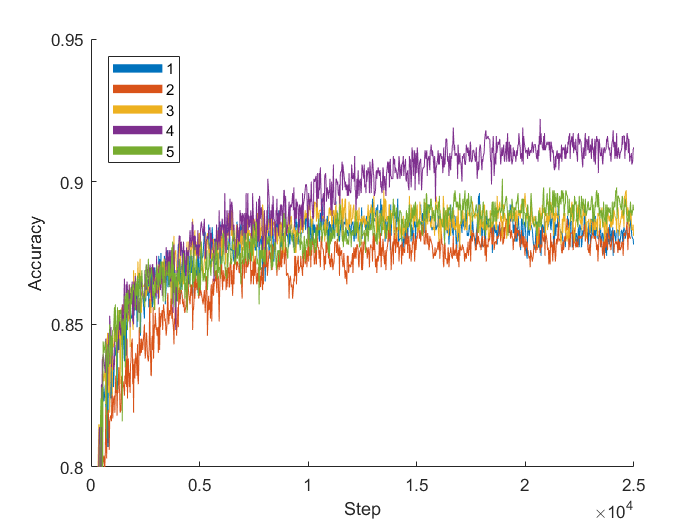
\includegraphics[width=8cm]{FC.png} }}
    \qquad
    \subfloat[Validation accuracy with varied LSTM timesteps (shown in legend)]{{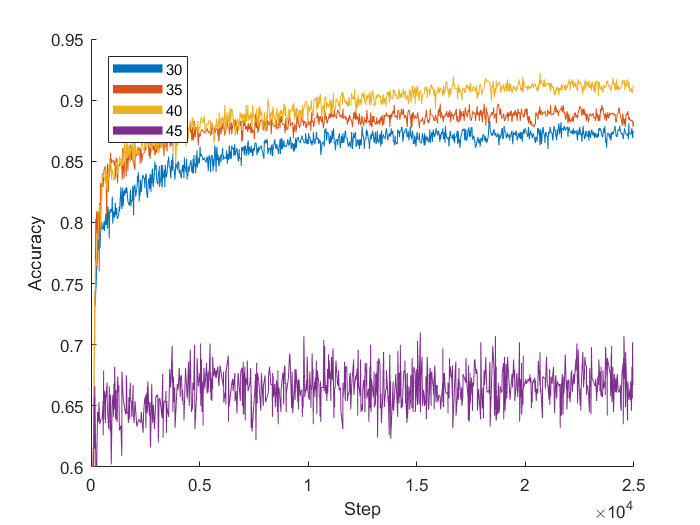
\includegraphics[width=8cm]{lstm.png} }}
    \caption{Validation accuracy plots for (a) varied numbers of fully connected layers and (b) varied LSTM timesteps}%
    \label{fig:accuracy}
\end{figure*}

\section{Conclusion}
We have presented a model for twitter sentiment analysis using LSTM neural network. In this project, we figure out that the challenge in preprocessing tweets is mostly related to variety form of word or speech, e.g. 'idk' is 'i do not know'. We do not investigate the following in our experiments but we believe it may improve the performance. In addition, we also do not analyze the structure of sentences. For example, although we map 'hate' to 'negative', the sentence could have been 'I do not hate', so it actually has positive sentiment. Then, we note that our implementation requires the LSTMs to receive a fixed number of words. Improvements in accuracy might be possible if we allow the LSTM timesteps to vary according to the number of words in each tweet.

\bibliographystyle{IEEEtran}
\bibliography{sample}

\end{document}
